\chapter{Problemy programowania liniowego}\label{ch:linearprog}
\thispagestyle{chapterBeginStyle}





Chcąc podjąć próbę formalnego opisania przedstawionych wcześniej problemów, należy najpierw zapoznać się z~ogólnymi zasadami ich zapisywania.
Jak mogliśmy zaobserwować w~poprzednim rozdziale, opisując problem typu \textsc{Incremental}, uciekliśmy się do przedstawienia go za pomocą serii nierówności oraz równości (\ref{mod:lpmodel1})~--- innymi słowy zapisaliśmy go w~postaci \textbf{modelu programowania liniowego}.
Możliwość przekształcenia dowolnie zadanego problemu do takiej postaci może nam zagwarantować odnalezienie jego istniejącego rozwiązania w~czasie wielomianowym i~takie narzędzie może stanowić doskonały punkt wyjściowy do dalszych rozważań.
W tym rozdziale omówimy ten sposób podejścia do problemów oraz przedstawimy narzędzia, które posłużą nam do konstrukcji algorytmu, rozwiązującego problem odpornej optymalizacji dla wyszukiwania minimalnego drzewa rozpinającego w~wersji \textsc{Incremental}, w rozdziale następnym.
Po drodze przedstawimy także alternatywne sposoby na radzenie sobie z problemami \textsc{MST} oraz \textsc{IMST}.




\section{Programowanie liniowe}




Mając na uwadze, że nie chcemy zajmować się zagadnieniem programowania liniowego samym w~sobie, gdyż nie jest to naszym celem, w~poniższym rozdziale zostaną przytoczone tylko podstawowe fakty, niezbędne do zrozumienia dalszej jego części.
Punktem wyjścia do pozyskania głębszej wiedzy na poruszany w~tym rozdziale temat może być książka~\cite{Papadimitriou:1982:COA:31027}, która omawia wszystkie aspekty tej dziedziny, począwszy od programowania wklęsłego, przez liniowe, do całkowitoliczbowego, tłumacząc zasady działania każdego z~tych modeli.

Przez pojęcie \textbf{programowania liniowego} będziemy rozumieli zbiór liniowych równań oraz nierówności wraz z~określoną dla nich \textbf{funkcją celu}, która także musi przybrać formę liniowego wyrażenia arytmetycznego.
Zbiór tych ograniczeń wraz z~funkcją celu będziemy nazywali \textbf{modelem prymalnym}\footnote{
	Terminem ,,prymalny'' będziemy określać modele programowania liniowego/całkowitoliczbowego, których funkcja celu jest minimalizacyjna.
	Problemem \textbf{dualnym} nazwiemy model, który skupia się na maksymalizowaniu jej wartości.
	Zagadnienia związane z~obydwoma modelami zostały dokładniej opisane w~książce~\cite[$67$--$73$]{Papadimitriou:1982:COA:31027}.
} programowania liniowego.
Schemat takiego modelu wygląda następująco:

\begin{subequations}
	\begin{alignat}{4}
	& \text{min} & & f \left( \textbf{x}, \dots \right)\textrm{,} &&& \\
	& \text{takie, że} & \quad & g_{1} \left( \textbf{x}, \dots \right) \quad \Diamond_{1} \quad b_{1}\textrm{,} && \text{(ang. \textit{subject to})}&\label{eq:lp:b} \\
	& & & g_{2} \left( \textbf{x}, \dots \right) \quad \Diamond_{2} \quad b_{2}\textrm{,} &&& \\
	& & & \cdots &&& \\
	& & & g_{m} \left( \textbf{x}, \dots \right) \quad \Diamond_{m} \quad b_{m}\textrm{,} &&&\label{eq:lp:d} \\
	& & & \phantom{\sum} x_{i} \geqslant x_{i}^{\textrm{LB}}, &\quad & & x_{i} \in \textbf{x}\textrm{,} \\
	& & & \phantom{\sum} x_{i} \leqslant x_{i}^{\textrm{UB}}, &\quad & & x_{i} \in \textbf{x}\textrm{,}
	\end{alignat}
\end{subequations}\label{eq:lp}
gdzie znak $\Diamond_{i}$ zastępuje dowolny znak ze zbioru $\left\{ =, \leqslant, \geqslant \right\}$, funkcja $f \left( \textbf{x}, \dots \right)$ jest funkcją celu i~przyjmuje postać $\sum_{i=1}^{n} c_{i} \cdot x_{i}$, $\textbf{x}$ jest wektorem symbolizującym rozwiązanie, $\textbf{c}$~--- zbiorem kosztów ($\left| \textbf{x} \right| = \left| \textbf{c} \right| = n$).
Zbiór funkcji $\left\{ g_{1} \left( \textbf{x}, \dots \right), \dots, g_{m} \left( \textbf{x}, \dots \right) \right\}$ oraz, odpowiadające im, wartości $\left\{ b_{1}, \dots, b_{m} \right\}$ będziemy zaś odpowiednio nazywać \textbf{ograniczeniami} modelu oraz \textbf{wartościami prawych stron}.
O~spełnieniu danej relacji $\Diamond_{i}$ przez parę $\left( g_{i} \left( \textbf{x}, \dots \right), b_{i} \right)$ będziemy mówić, że zaszło ograniczenie $i$~--- oczywiście rozwiązanie dowolnego modelu jest dopuszczalne tylko wtedy, gdy spełnia ono je wszystkie.
Wektor $\textbf{x}$ będziemy nazywać zbiorem \textbf{zmiennych decyzyjnych} modelu.
Dla wszystkich do tej pory opisanych problemów w~poprzednim rozdziale wykorzystywaliśmy podobne oznaczenia~--- zmienna decyzyjna $x_{i}$ przyjmowała odpowiednio wartość $0$, gdy krawędź $e_{i}$ nie należała do poszukiwanego rozwiązania, oraz $1$ w~przeciwnym przypadku.
Tutaj generalizujemy tę ideę, dopuszczając przyjmowanie przez te zmienne wartości z~zakresu od $x_{i}^{\textrm{LB}}$ do $x_{i}^{\textrm{UB}}$, gdzie odpowiednio $x_{i}^{\textrm{LB}}$ oznacza dolne ograniczenie na wartość zmiennej $x_{i}$ (ang. \textit{lower bound}), zaś $x_{i}^{\textrm{UB}}$~--- górne (ang. \textit{upper bound}).
Od rodzaju wartości, jakie mogą przyjmować te zmienne, zależy z~jakiego typu problemem mamy do czynienia~--- w~przypadku, gdy wartości $x_{i} \in \left\langle x_{i}^{\textrm{LB}}, x_{i}^{\textrm{UB}} \right\rangle$, model, w~którym występują tylko takie zmienne, będziemy nazywali modelem programowania liniowego (ang. \textsc{LP}~--- \textit{Linear Programming}).
W~przeciwnym przypadku, gdy w~modelu pojawią się zmienne o~wartościach dyskretnych ($x_{i} \in \left[ x_{i}^{\textrm{LB}}, x_{i}^{\textrm{UB}} \right]$), mówimy o~modelu \textbf{całkowitoliczbowym} (ang. \textsc{IP}~--- \textit{Integer Programming}).
Ma to o~tyle duże znaczenie, że w~pierwszym przypadku jesteśmy w~stanie zagwarantować, że o~ile dla zdefiniowanego modelu istnieje \textbf{rozwiązanie optymalne} (minimalizujące funkcję celu $f \left( \textbf{x}, \dots \right)$), otrzymamy je w~czasie wielomianowym od wielkości modelu.
Informację o~braku takiego rozwiązania również uzyskamy w~takim czasie (często dużo szybciej, gdy algorytm, służący do rozwiązywania tak zdefiniowanych problemów, znajdzie się w~stanie, który będzie tożsamy z~brakiem istnienia jakiegokolwiek rozwiązania\footnote{
	Dla przykładu: ograniczenia w~postaci funkcji $g \left( \textbf{x}, \dots \right)$ mogą tak ograniczyć zbiór wartości, które może przyjąć dana zmienna decyzyjna $x_{i}$, że w~pewnym momencie $x_{i} \in \emptyset$ (co jest sygnałem dla algorytmu, że dalsze obliczenia są bezcelowe).
}).
W~przypadku zaś modeli całkowitoliczbowych nie mamy takiej gwarancji\footnote{
	Algorytm rozwiązujący dany problem w~pierwszej kolejności znajdzie rozwiązanie problemu, ignorując ograniczenia na całkowitoliczbowość zmiennych decyzyjnych, a~następnie zacznie szukać takiego rozwiązania, które będzie je spełniać, będąc jednocześnie rozwiązaniem możliwie najlepszym.
	W~wielu przypadkach kończy się to na inteligentnym przeglądaniu wszystkich możliwych rozwiązań metodą np. podziału i~ograniczeń (ang. \textit{branch and bound})~\cite[$433$--$448$]{Papadimitriou:1982:COA:31027}.
} i~często czas, potrzebny do znalezienia rozwiązania, wykracza poza wielomianowy.
W~przypadku gdy w~modelu występują oba typy zmiennych, mamy do czynienia z~modelem mieszanym \textbf{MIP} (ang. \textit{Mixed Integer Programming}), którego czas rozwiązania również może być ponad-wielomianowy.
Aby zilustrować działanie tak opisanego modelu, wyjaśnić jak go należy rozumieć, posłużymy się poniższym przykładem, który ukazuje rzeczywisty model (\ref{fig:lpexample:a}), który w kolejnych krokach (\ref{fig:lpexample:b} i \ref{fig:lpexample:c}) sprowadzimy do, przedstawionego wcześniej, schematu.

\begin{figure}[!htbp]
	\renewcommand\figurename{Model}
	\null\hfill
	\begin{subfigure}[b]{0.3\textwidth}
		\begin{subequations}
			\begin{alignat*}{4}
			& \text{min} & & 2 \cdot x_{1} + 3 \cdot x_{2}\textrm{,} &&&\\
			& \text{s.t.} & \quad & 3 \cdot x_{1} + 2 \cdot x_{2} \leqslant 12\textrm{,} &&&\\
			& & \quad & 1 \cdot x_{1} - 4 \cdot x_{2} \geqslant 2\textrm{,} &&&\\
			& & & \phantom{\sum} 0 \leqslant x_{1} \leqslant 3, &\quad & x_{i} &\in \textbf{x}\textrm{,} \\
			& & & \phantom{\sum} 0 \leqslant x_{2} \leqslant 4, &\quad & x_{i} &\in \textbf{x}\textrm{.}
			\end{alignat*}
		\end{subequations}
		\caption{}
		\label{fig:lpexample:a}
	\end{subfigure}
	\hfill
	\begin{subfigure}[b]{0.3\textwidth}
		\begin{gather*}
		f \left( \textbf{x}, \textbf{c} \right) = \sum_{i=1}^{i=2} c_{i} \cdot x_{i}\textrm{,}\\
		g_{1} \left( \textbf{x}, \textbf{a}_{1} \right) = \sum_{i=1}^{i=2} a_{1,i} \cdot x_{i}\textrm{,}\\
		g_{2} \left( \textbf{x}, \textbf{a}_{2} \right) = \sum_{i=1}^{i=2} a_{2,i} \cdot x_{i}\textrm{.}
		\end{gather*}
		\caption{}
		\label{fig:lpexample:b}
	\end{subfigure}
	\hfill
	\begin{subfigure}[b]{0.3\textwidth}
		\begin{subequations}
			\begin{alignat*}{4}
			& \text{min} & & f \left( \textbf{x}, \textbf{c} \right)\textrm{,} &&&\\
			& \text{s.t.} & \quad & g_{1} \left( \textbf{x}, \textbf{a}_{1} \right) \leqslant b_{1}\textrm{,} &&&\\
			& & \quad & g_{2} \left( \textbf{x}, \textbf{a}_{2} \right) \geqslant b_{2}\textrm{,} &&&\\
			& & & \phantom{\sum} 0 \leqslant x_{1} \leqslant 3, &\quad & x_{i} &\in \textbf{x}\textrm{,} \\
			& & & \phantom{\sum} 0 \leqslant x_{2} \leqslant 4, &\quad & x_{i} &\in \textbf{x}\textrm{.}
			\end{alignat*}
		\end{subequations}
		\caption{}
		\label{fig:lpexample:c}
	\end{subfigure}
	\hfill\null
	\caption{
		Przykładowy problem sformułowany jako model programowania liniowego.
		\textbf{(a)}~Jawnie zapisany model~--- w~takiej formie będzie rozwiązywany przez wyspecjalizowany algorytm do rozwiązywania zagadnień programowania liniowego.
		\textbf{(b)}~Reprezentacja wszystkich elementów modelu w~zwartej formie funkcji z~następująco zdefiniowanymi zbiorami wartości: $\textbf{x} = \left\{ x_{1}, x_{2} \right\}$, $x_{1} \in \left\langle 0, 3 \right\rangle$, $x_{2} \in \left\langle 0, 4 \right\rangle$, $\textbf{c} = \left[ 2, 3 \right]$, $\textbf{b} = \left[ 12, 2 \right]$, $\textbf{a}_{1} = \left[ 3, 2 \right]$ i~$\textbf{a}_{2} = \left[ 1, -4 \right]$.
		\textbf{(c)}~Zwarty zapis modelu.
	}
	\label{fig:lpexample}
\end{figure}

Oczywistym rozwiązaniem problemu \ref{fig:lpexample} jest para wartości $\left( 2, 0 \right)$.
Przypisanie takich liczb do zmiennych $x_{1}$ oraz $x_{2}$ spełnia wszystkie ograniczenia zawarte w~modelu, wartości przypisane zmiennym należą do ich dziedzin, zaś wartość funkcji celu dla tak zadanych zmiennych osiąga swoje minimum.
Zwykle możemy spotkać się z~macierzowym zapisem modelu, gdzie przedstawione przez nas wektory $\textbf{a}_{1}$ oraz $\textbf{a}_{2}$ traktuje się jako macierz $A = \left[ \textbf{a}_{1}, \textbf{a}_{2} \right]^{T}$ a~układ ograniczeń zadanego modelu prezentuje się w~postaci $A \cdot \textbf{x} = \textbf{b}$.



\subsection{Problem minimalnego drzewa rozpinającego}



W dalszej części rozdziału poznamy szereg różnych modeli, przedstawiających problem minimalnego drzewa rozpinającego, poczynając od bezpośredniej próby przełożenia jego definicji na model matematyczny, poprzez modele całkowitoliczbowe, aż do modelu programowania liniowego, którego specyficzna budowa zapewni nam całkowitoliczbowe rozwiązanie.
Na tej podstawie będziemy chcieli skonstruować modele odpowiadające problemowi minimalnego drzewa rozpinającego w~wersji \textsc{Incremental}, które posłużą nam jako punkt wyjścia do dalszych rozważań.



\subsection{Naiwne podejście}



Pierwszym i~zarazem najbardziej naturalnym sposobem podejścia do zamodelowania interesującego nas problemu jest model przedstawiony poniżej.
Opiera się on na ogólnie znanych właściwościach drzew rozpinających i~ich podstruktury~--- jeśli dane drzewo $T$ jest drzewem rozpinającym dla grafu $G = \left( V, E \right)$ (między innymi składa się z~$\left| V \right| - 1$ krawędzi), to każdy podzbiór wierzchołków $S \subseteq V$ grafu jest połączony ze sobą co najwyżej $\left| S \right| - 1$ krawędziami (zobacz rysunek \ref{fig:mst1Example:a}).
Niech zbiór $E \left( S \right)$ będzie zdefiniowany jako $E \left( S \right) = \left\{ \left\{ i, j \right\} : v_{i} \overset{1}\leadsto v_{j} \in E \; \wedge \; v_{i} \in S \; \wedge \; v_{j} \in S \right\}$ i~oznacza zbiór wszystkich krawędzi łączących dowolne dwa różne wierzchołki ze zbioru $S$.
Niech dodatkowo dla każdej krawędzi w~grafie $e \in E$ będzie zdefiniowana zmienna decyzyjna $x_{e}$, której wartość odpowiada decyzji o~przynależności danej krawędzi do minimalnego drzewa rozpinającego, będącego rozwiązaniem $T$ dla modelu \ref{mod:mst1} (innymi słowy, minimalne drzewo rozpinające $T$ składa się z~krawędzi $e$, dla których $x_{e} = 1$~--- $T = \left\{ e : x_{e} = 1 \right\}$).
W~takiej sytuacji równanie \ref{eq:modmst1:c} w~naturalny sposób opisuje wskazaną przez nas własność.
W~szczególności dla zbioru $S = V$ mamy $E \left( S \right) = E$, a~wspomniane równanie sprowadza się do wyrażenia \ref{eq:modmst1:b}, które w~dobitny sposób wyraża podstawową własność, posiadaną przez drzewa rozpinające dowolny graf.
Teraz, aby uzyskać minimalne takie drzewo, wystarczy byśmy zdefiniowali funkcję celu, która będzie dążyć do zminimalizowania kosztów znalezionego rozwiązania (\ref{eq:modmst1:a}).

\begin{figure}[!h]
	\null\hfill
	\begin{subfigure}[b]{0.36\textwidth}
		\includegraphics[width=\textwidth]{Chapter_III/MST1-example/a}
		\caption{}
		\label{fig:mst1Example:a}
	\end{subfigure}
	\hfill
	\begin{subfigure}[b]{0.5\textwidth}
		\begin{subequations}
			\begin{alignat}{4}
			& \text{min} & & \sum_{\mathclap{e \in E}} c_{e} \cdot x_{e}\textrm{,}\label{eq:modmst1:a} \\
			& \text{s.t.} & \quad & \sum_{\mathclap{e \in E}} x_{e} = \left| V \right| - 1\text{,}\label{eq:modmst1:b} \\
			& & & \sum_{\mathclap{e \in E \left( S \right) }} x_{e} \leqslant \left| S \right| - 1, & \quad & S & \subseteq V\textrm{,}\label{eq:modmst1:c} \\
			& & & \phantom{\sum} x_{e} \geqslant 0, &\quad & e &\in E\textrm{.}
			\end{alignat}
		\end{subequations}
		\caption{}
		\label{fig:mst1Example:b}
		\label{mod:mst1}%Obie referencje są używane, żeby się nie myliło, gdy mowa o modelu a o subfigurze
	\end{subfigure}
	\hfill\null
	\caption{
		Minimalne drzewo rozpinające, uzyskane za pomocą, przedstawionego obok, modelu programowania liniowego.
		\textbf{(a)}~Przykładowe drzewo rozpinające $T = \left\{ e_{1}, e_{3}, e_{4}, e_{6}, e_{9} \right\}$ dla grafu $G = \left( V, E \right)$.
		Dla dowolnego podzbioru $S \subseteq V$ liczba krawędzi $\left\{ e_{ij} : e_{ij} \in T \; \wedge \; v_{i} \in S \; \wedge \; v_{j} \in S \right\}$ jest co najwyżej równa $\left| S \right| - 1$ (żaden podzbiór $S \subseteq V$ wraz z odpowiadającymi mu krawędziami $E \left( S \right)$ nie tworzy cykli~--- innymi słowy każdy graf $G_{S} = \left( S, E \left( S \right) \right)$ jest acykliczny).
		\textbf{(b)}~Model liniowego programowania dla problemu minimalnego drzewa rozpinającego.
	}
	\label{fig:mst1Example}
\end{figure}

Niestety model, którego idea wydaje się być bardzo prosta, jest równie intuicyjny co niepraktyczny w~zastosowaniu.
Wystarczy spojrzeć na definicję zbioru $E \left( S \right)$ bądź na rysunek \ref{fig:mst1Example:a} oraz jego opis, by dojść do wniosku, że liczba wymaganych przez model ograniczeń jest ponad-wielomianowa~--- znacznie większa niż czas, w~którym spodziewalibyśmy się otrzymać rozwiązanie dla takiego modelu programowania liniowego (przypomnijmy, że modelem \textsc{LP} nazywamy model, którego zmienne decyzyjne nie są ograniczone do dyskretnego zbioru liczb)\footnote{
	Z wiedzy ogólnej wiemy, że wszystkich podzbiorów zbioru, składającego się z~$n$ elementów, jest $2^{n}$ ($\sum_{i=0}^{n} \binom{n}{i}$).
	Wzór ten doskonale opisuje naszą sytuację~--- chcemy mieć ograniczenie dla wszystkich możliwych zbiorów $S$ jedno-, dwu-, $\dots$, $n$-elementowych.
	Z~drugiej zaś strony powiedzieliśmy (rozdzielając pojęcia programowania liniowego od całkowitoliczbowego), że wykorzystanie modelu \textsc{LP} gwarantuje nam możliwość otrzymania jego rozwiązania w~czasie wielomianowym \textbf{od rozmiaru problemu}.
	W~związku z~czym algorytm, rozwiązujący dany model, będzie zwracał interesujący nas wynik w~nieakceptowalnym dla nas czasie.
	Aby mimo wszystko uzyskać chciane rozwiązanie w~czasie wielomianowym, musimy zrezygnować z~algorytmów, które czasem działania płacą za swoją uniwersalność (taki jak przez nas przyjęty algorytm \textsc{simplex}~\cite{Gass2011}, którym potrafimy rozwiązać dowolne zagadnienie z~\textsc{LP}), na rzecz bardziej złożonych metod, które do działania nie potrzebują pełnego opisu problemu, tak jak wspomniany przez nas algorytm (a zatem ich czas działania nie jest na samym początku ograniczony z~dołu wielkością zadanego modelu, lecz występującą w~nim liczbą zmiennych decyzyjnych, a~tych w~omawianym przypadku jest niewiele~--- $\left| E \right|$)~\cite{DBLP:conf/icalp/BeiCZ15}.
}



\subsection{Przepływy}



Innym sposobem podejścia do problemu minimalnego drzewa rozpinającego jest jego zdefiniowanie za pomocą \textbf{przepływów}~\cite[$38$--$44$]{Magnanti1995503}.
W~tej interpretacji węzłami są miejsca, w~których dozwolony jest skład pewnych towarów, zaś krawędzie między nimi symbolizują ścieżki, którymi dane towary możemy przemieszczać pomiędzy dwoma sąsiednimi punktami, ponosząc tego koszty proporcjonalnie do wagi wybranej krawędzi, która je łączy.
Załóżmy, że mamy dany graf $G$, taki jak przedstawiono na rysunku \ref{fig:mst2Example}.
Dodatkowo niech jeden z~węzłów w~grafie ($v_{1}$) będzie wyróżniony i~posiada tyle jednostek towarów, ile w~grafie jest wierzchołków.
Naszym celem jest dystrybucja wszystkich towarów z~wykorzystaniem dostępnych krawędzi w~taki sposób, aby każdy z~transportów dotarł w~efekcie końcowym do innego wierzchołka~--- biorąc pod uwagę, że życzymy sobie, aby przy okazji ponieść tego jak najmniejsze koszty, okaże się że droga, która zostanie w~ten sposób wytyczona z~punktu startowego $v_{1}$ do wszystkich $v_{j} \in V \setminus \left\{ v_{1} \right\}$, jest minimalnym drzewem rozpinającym ten graf, a~fakt rozdzielenia towarów pomiędzy wszystkie węzły w~oczywisty sposób świadczy o~spójności tak wygenerowanego drzewa.

\begin{figure}[!htbp]
	\null\hfill
	\begin{subfigure}[b]{0.254\textwidth}
		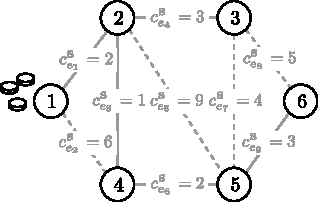
\includegraphics[width=\textwidth]{Chapter_III/MST2-example/a}
		\caption{}
		\label{fig:mst2Example:a}
	\end{subfigure}
	\hfill
	\begin{subfigure}[b]{0.242\textwidth}
		\includegraphics[width=\textwidth]{Chapter_III/MST2-example/b}
		\caption{}
		\label{fig:mst2Example:b}
	\end{subfigure}
		\hfill
	\begin{subfigure}[b]{0.242\textwidth}
		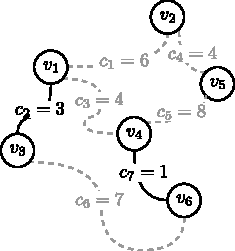
\includegraphics[width=\textwidth]{Chapter_III/MST2-example/c}
		\caption{}
		\label{fig:mst2Example:c}
	\end{subfigure}
	\hfill
	\begin{subfigure}[b]{0.242\textwidth}
		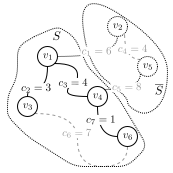
\includegraphics[width=\textwidth]{Chapter_III/MST2-example/d}
		\caption{}
		\label{fig:mst2Example:d}
	\end{subfigure}
	\hfill\null
	\caption{
		Rysunek przedstawiający wygenerowany przepływ dla problemu znalezienia minimalnego drzewa rozpinającego.
		Szarymi ciągłymi liniami zostało zaznaczone optymalne rozwiązanie problemu, przerywanymi~--- pozostałe krawędzie w~grafie, zaś czarnymi oznaczone są łuki, które do tej pory były wykorzystane do transportu towarów.
		\textbf{(a)}~Sytuacja początkowa z~wszystkimi pięcioma elementami zgromadzonymi przy węźle $v_{1}$.
		\textbf{(b)}~Z wierzchołka $v_{1}$ została przekazana piątka elementów z~wykorzystaniem krawędzi $e_{1}$.
		\textbf{(c)}~Z wierzchołkiem $v_{2}$ połączone są jeszcze dwie krawędzie należące do minimalnego drzewa rozpinającego danego grafu przy tak zdefiniowanych kosztach~--- wykorzystując krawędzie $e_{3}$ oraz $e_{4}$, do nowych wierzchołków zostały w~sumie przemieszczone cztery elementy, pozostawiając jeden w~wierzchołku $v_{2}$.
		\textbf{(d)}~W wyniku rozdystrybuowania wszystkich elementów tak, aby każdy wierzchołek posiadał dokładnie jeden spośród nich, otrzymano minimalne drzewo rozpinające dla prezentowanego grafu. 
	}
	\label{fig:mst2Example}
\end{figure}

Niech teraz z~każdą krawędzią $e_{ij}$ ($e_{ij} \equiv v_{i} \overset{1}{\leadsto} v_{j} \; \wedge \; v_{j} \overset{1}{\leadsto} v_{i}$) będą związane dwie dodatkowe zmienne: $f_{ij}$ oraz $f_{ji}$, symbolizujące przepływ (ang. \textit{flow}) na tej krawędzi w~danym kierunku (wartość zmiennej $f_{ij}$ oznacza więc liczbę elementów, które z~wierzchołka $v_{i}$ przesunęliśmy do $v_{j}$ przy wykorzystaniu krawędzi $e_{ij}$, zaś zmienna $f_{ji}$ symbolizuje odwrotną zależność~--- liczbę transportowanych elementów po tym samym łuku, lecz z~$v_{j}$ do $v_{i}$).
Tak jak to sobie powiedzieliśmy i~jak mogliśmy zaobserwować na rysunku \ref{fig:mst2Example:a}, naszym celem jest wyjście z~sytuacji, gdzie w~jednym wierzchołku znajduje się $n = \left| V \right|$ elementów, i~zakończenie w~takiej, w~której do każdego wierzchołka przyporządkowany jest jeden z~nich~--- innymi słowy chcemy, aby z~wyróżnionego wierzchołka wysłanych zostało $n - 1$ posiadanych przez niego elementów, przy jednoczesnym upewnieniu się, że żaden z~nich do niego nie wróci.
W~równaniu \ref{eq:mst2:flowArray} możemy wyróżnić dwie sumy, które kolejno oznaczają:

\begin{itemize}
	\item $\sum_{ \left( i, j \right ) \in E } f_{ij}$~--- sumę wartości wszystkich przepływów, których kierunek jest wyznaczony w~stronę wierzchołków innych niż $v_{i}$ (mówimy wtedy o~sumie przepływów \textbf{wyjściowych} wierzchołka $v_{i}$),
	\item $\sum_{ \left( j, i \right ) \in E } f_{ji}$~--- sumę wartości przepływów skierowanych w~stronę wierzchołka $v_{i}$ (sumę przepływów przychodzących do danego wierzchołka).
\end{itemize}

Innymi słowy wartość pierwszego wyrażenia będzie równa liczbie ładunków, które wysłaliśmy z~wierzchołka $v_{i}$ do pozostałych węzłów, zaś wartość drugiej sumy oznacza liczbę tych ładunków, które do wierzchołka $v_{i}$ dotarły.
Widzimy zatem, że wartość wyrażenia z~równania \ref{eq:mst2:flowArray} dla parametru $i = 1$ odpowiada opisanej przez nas sytuacji~--- wierzchołek początkowy wysyła w~kierunku pozostałych wierzchołków łącznie $n - 1$ ładunków (sobie pozostawiając jeden~--- $\sum_{ \left( 1, j \right ) \in E } f_{1j} = n - 1$), zaś sam nie przyjmuje żadnych~--- $\sum_{ \left( j, 1 \right ) \in E } f_{j1} = 0$.
Dla wszystkich pozostałych przypadków, tak jak to mogliśmy zaobserwować na rysunkach \ref{fig:mst2Example:a}--\ref{fig:mst2Example:d}, każdy wierzchołek, z~otrzymanych od sąsiada elementów, wybierał dla siebie jeden a~resztę przekazywał dalej, co natychmiast prowadzi do równości $\sum_{ \left( j, i \right ) \in E } f_{ji} - \sum_{ \left( i, j \right ) \in E } f_{ij} = 1$ (i oczywiście $\sum_{ \left( i, j \right ) \in E } f_{ij} - \sum_{ \left( j, i \right ) \in E } f_{ji} = -1$, gdyż w~takiej formie najwygodniej jest nam zastosować tą równość w~prezentowanym modelu \ref{mod:mst2}~\cite[$35$]{robustSTP}).

\begin{subequations}
	\begin{alignat}{4}
	& \text{min} & & \sum_{\mathclap{e \in E}} c_{e} \cdot x_{e}\text{,}\label{mod:mst2:a} \\
	& \text{s.t.} & \quad & \sum_{\mathclap{ \left( i, j \right ) \in E }} f_{ij} - \sum_{\mathclap{ \left( j, i \right ) \in E }} f_{ji} &= \left\{
	\begin{matrix}
		n - 1 & \text{jeżeli}~i = 1 \text{,}\\ 
		-1 & \text{w przeciwnym przypadku,}
	\end{matrix}\label{eq:mst2:flowArray}
	\right.\\
	& & & f_{ij} \leqslant \left( n - 1 \right) \cdot x_{ij}, & \forall  \left\{ i, j \right\} \in E\text{,}&&&\label{eq:mst2:flow1}\\
	& & & f_{ji} \leqslant \left( n - 1 \right) \cdot x_{ij}, & \forall  \left\{ i, j \right\} \in E\text{,}&&&\label{eq:mst2:flow2}\\
	& & & \sum_{\mathclap{e \in E}} x_{e} = n - 1\text{,} & & &\\
	& & & \phantom{\sum} f_{e} \geqslant 0\text{,} & \forall e \in E\text{,}\label{mod:mst2:f}&&&\\
	& & & \phantom{\sum} x_{e} \in \left\{ 0, 1 \right\}\text{,} & \forall e\in E\text{.}\label{mod:mst2:g}&&&
	\end{alignat}\label{mod:mst2}
\end{subequations}

Reszta ograniczeń w~modelu \ref{mod:mst2} wydaje się być intuicyjna~--- poprzez ograniczenia takie jak \ref{eq:mst2:flow1} czy \ref{eq:mst2:flow2} gwarantujemy sobie, że w~przypadku krawędzi $e$, która należy do minimalnego drzewa rozpinającego ($x_{e} = 1$), liczba przesyłanych przezeń elementów wynosić może maksymalnie $n - 1$ (czyli tyle, ile przesyłałby wierzchołek początkowy, gdyby posiadał tylko jednego sąsiada), w~przeciwnym zaś razie wykorzystanie tej krawędzi jest zabronione ($x_{ij} = 0 \rightarrow f_{ij} = 0$).
Dodatkowo posiadamy ograniczenie, które determinuje liczbę krawędzi tworzących rozwiązanie, oraz ograniczenia wartości samych zmiennych decyzyjnych.
Te ostatnie widzimy, że ograniczają ich dziedzinę do jedynie dwóch wartości ($0$ oraz $1$), co wskazuje na to, że przedstawiony w~\ref{mod:mst2} model opisuje problem programowania całkowitoliczbowego, w~związku z~czym oczekiwany czas otrzymania rozwiązania tak postawionego problemu, przy wykorzystaniu naszego modelu \ref{mod:mst2}, nie jest w~żaden sposób z góry ograniczony funkcją wielomianową od wielkości problemu.
Możemy oczywiście zignorować ograniczenia całkowitoliczbowości, licząc na prawidłowe zachowanie się modelu bez tego ograniczenia~--- choć brzmi to niedorzecznie, w~rzeczywistości (np. dla grafu i~kosztów zaprezentowanych na rysunkach \ref{fig:mst2Example:a}--\ref{fig:mst2Example:d}) może się okazać, że otrzymamy identyczne rozwiązanie co w~przypadku zastosowania ograniczeń na całkowitoliczbowość, co może sugerować, że tak zbudowany model również jest poprawny.

\begin{figure}[!h]
	\null\hfill
	\begin{subfigure}[b]{0.27\textwidth}
		\includegraphics[width=\textwidth]{Chapter_III/MST3-example/a}
		\caption{}
		\label{fig:mst3Example:a}
	\end{subfigure}
	\hfill
	\begin{subfigure}[b]{0.27\textwidth}
		\includegraphics[width=\textwidth]{Chapter_III/MST3-example/b}
		\caption{}
		\label{fig:mst3Example:b}
	\end{subfigure}
	\hfill\null
	\caption{
		Optymalne rozwiązania dla modelu przedstawionego w~\ref{mod:mst2}.
		\textbf{(a)}~Minimalne drzewo rozpinające o~całkowitym koszcie $2$, zwrócone przez model opisany ograniczeniami \ref{mod:mst2:a}--\ref{mod:mst2:g}.
		Wartości zmiennych decyzyjnych $\left\{ x_{i} : e_{i} \in E \right\}$ są ograniczone do wartości $0$ (krawędź nie należy do rozwiązania) albo $1$.
		\textbf{(b)}~Rozwiązanie nie będące drzewem rozpinającym, zwrócone przez model opisany ograniczeniami \ref{mod:mst2:a}--\ref{mod:mst2:f} (gdzie dodatkowo $\forall e_{i} \in E \; : \; x_{i} \geqslant 0$).
	}
	\label{fig:mst3Example}
\end{figure}

Niestety, jak widzimy na rysunkach \ref{fig:mst3Example:a} oraz \ref{fig:mst3Example:b}~\cite[$41$]{Magnanti1995503}, nawet w~najprostszych przypadkach zniesienie wspomnianego ograniczenia może spowodować, że zwracane rozwiązania będą niedopuszczalne w~myśl problemu minimalnego drzewa rozpinającego (choć oczywiście wszystkie ograniczenia tak zbudowanego modelu są spełnione~--- po prostu nie modeluje on już więcej problemu, którego rozwiązania byśmy oczekiwali~\cite[$39$]{Magnanti1995503}).
W~związku z~tym będziemy chcieli zaproponować trzeci wariant rozwiązania, który w~znacznym stopniu opiera się na idei powyższego modelu, jednak w~odróżnieniu od swojego poprzednika, optymalne rozwiązania przez niego zwracane będą poprawne nawet, jeżeli zaniechamy ograniczenia na całkowitoliczbowość zmiennych decyzyjnych $\left\{ x_{i} : e_{i} \in E \right\}$.



\subsection{Przepływy z~całkowitymi punktami ekstremalnymi}



W tej części będziemy chcieli pokazać wariację na temat poprzednio prezentowanego modelu (patrz model \ref{mod:mst2}), która pozwoli nam na stwierdzenie, że dla tak zbudowanego modelu, jego rozwiązania (punkty ekstremalne~\cite{Papadimitriou:1982:COA:31027}) są liczbami całkowitymi~\cite[$42$--$46$]{Magnanti1995503}, bez względu na to, jakie ograniczenia zostaną nałożone na zmienne decyzyjne tego modelu.
To z~kolei pozwoli nam na zdefiniowanie dziedzin wszystkich zmiennych decyzyjnych jako nieograniczonego zakresu liczb rzeczywistych większych od zera~--- z~omówionych wcześniej własności problemu modelowania wiemy zaś, że w~takim przypadku mamy do czynienia z~modelem programowania liniowego, rozwiązywalnego w~czasie wielomianowym (a to jest właśnie naszym celem~--- pokazanie modelu, dla którego rozwiązanie otrzymamy w~opisanym przez nas czasie).
Zanim jednak przedstawimy pełen model (\ref{mod:mst3}), zaproponowany w~\cite[$42$--$46$]{Magnanti1995503}, omówimy kolejno znaczenie wszystkich najistotniejszych jego ograniczeń, które wymagają pochylenia się nad nimi.


\subsubsection{Wielotowarowy model przepływu dla grafów skierowanych} 


Zasadniczą różnicą pomiędzy tym (ang. \textit{directed multicommodity flow model}) a~poprzednio przedstawionym modelem jest odmienny sposób organizacji przepływu pomiędzy wierzchołkami grafu.
Spójrzmy na rysunki \ref{fig:mst4Example:a}--\ref{fig:mst4Example:d}~--- przedstawiają one niemal tę samą sytuację co na rysunku \ref{fig:mst2Example}, lecz skupiają się one jedynie na pojedynczym elemencie do przetransportowania, w~odróżnieniu od przytoczonego przykładu.

\begin{subequations}
	\begin{alignat}{4}
	& \text{min} & & \sum_{ \left( i, j \right) \in E} c_{ij} \cdot \left( y_{ij} + y_{ji} \right)\text{,} \\
	& \text{s.t.} & \quad & \sum_{\mathclap{ \left( j, s \right ) \in E }} f^{k}_{js} - \sum_{\mathclap{ \left( s, j \right ) \in E }} f^{k}_{sj} = -1, & \forall v_{k} \in V \setminus \left\{ v_{s} \right\}\text{,}\label{mod:mst3:b}\\
	& & & \sum_{\mathclap{ \left( j, i \right ) \in E }} f^{k}_{ji} - \sum_{\mathclap{ \left( i, j \right ) \in E }} f^{k}_{ij} = 0\text{,} & \forall v_{i}, v_{k} \in V \setminus \left\{ v_{s} \right\} \; \wedge \; i \neq k\text{,}\label{mod:mst3:c}\\
	& & & \sum_{\mathclap{ \left( j, k \right ) \in E }} f^{k}_{jk} - \sum_{\mathclap{ \left( k, j \right ) \in E }} f^{k}_{kj} = 1\text{,} & \forall v_{k} \in V \setminus \left\{ v_{s} \right\}\text{,}\label{mod:mst3:d}\\
	& & & f^{k}_{ij} \leqslant y_{ij}, & \forall \left( i, j \right) \in E \; \wedge \; \forall v_{k} \in V \setminus \left\{ v_{s} \right\}\text{,}&&&\label{mod:mst3:e}\\
	& & & \sum_{\mathclap{ \left( i, j \right) \in E}} y_{ij} = n - 1\text{,} & & &\label{mod:mst3:f}\\
	& & & \phantom{\sum} f_{ij} \geqslant 0\text{,} & \forall \left( i, j \right) \in E\text{,}&&&\\
	& & & \phantom{\sum} y_{ij} \geqslant 0\text{,} & \forall \left( i, j \right) \in E\text{.}&&&
	\end{alignat}\label{mod:mst3}
\end{subequations}

\begin{figure}[!htbp]
	\null\hfill
	\begin{subfigure}[b]{0.254\textwidth}
		\includegraphics[width=\textwidth]{Chapter_III/MST4-example/a}
		\caption{}
		\label{fig:mst4Example:a}
	\end{subfigure}
	\hfill
	\begin{subfigure}[b]{0.242\textwidth}
		\includegraphics[width=\textwidth]{Chapter_III/MST4-example/b}
		\caption{}
		\label{fig:mst4Example:b}
	\end{subfigure}
	\hfill
	\begin{subfigure}[b]{0.242\textwidth}
		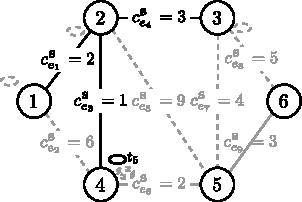
\includegraphics[width=\textwidth]{Chapter_III/MST4-example/c}
		\caption{}
		\label{fig:mst4Example:c}
	\end{subfigure}
	\hfill
	\begin{subfigure}[b]{0.242\textwidth}
		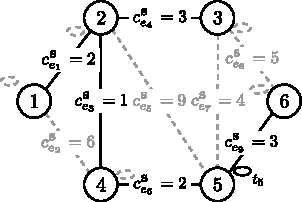
\includegraphics[width=\textwidth]{Chapter_III/MST4-example/d}
		\caption{}
		\label{fig:mst4Example:d}
	\end{subfigure}
	\hfill\null
	\caption{
		Przepływ towarów z~perspektywy wyróżnionego elementu $t_{5}$.
		\textbf{(a)}~Sytuacja początkowa: wierzchołkiem startowym jest wierzchołek $v_{1} = v_{s}$, końcowym dla wyróżnionego towaru~--- $v_{5}$.
		\textbf{(b)}~Towar $t_{5}$ został przesunięty w~kierunku następnego wierzchołka.
		Suma przepływów wychodzących dla danego towaru z~wierzchołka startowego wynosi $1$.
		Wszystkie wierzchołki pośrednie (nie będące ani początkowym, ani końcowym dla branego pod uwagę towaru), które otrzymują towar $t_{5}$ w~czasie jego drogi do $v_{5}$, otrzymawszy go,
		\textbf{(c)}~natychmiast przesyłają go dalej~--- bilans przepływu dla takiego wierzchołka względem towaru $t_{5}$ wynosi $0$.
		\textbf{(d)}~Różnica przepływów wchodzących oraz wychodzących do wierzchołka będącego odbiorcą swojego towaru wynosi $1$~--- jeśli wierzchołek nie jest wierzchołkiem początkowym, akceptuje on tylko przeznaczony dla siebie element, resztę zaś przesyła dalej w~chwili ich otrzymania (równość \ref{mod:mst3:d}).
	}
	\label{fig:mst4Example}
\end{figure}

Na wspomnianych rysunkach widzimy zatem wyraźnie sposób konstrukcji ograniczeń \ref{mod:mst3:b}, \ref{mod:mst3:c} oraz \ref{mod:mst3:d}.
Niech zmienne decyzyjne $f_{ij}$ oznaczają przepływ tak jak w~poprzednim modelu.
Wprowadźmy teraz nowe zmienne $f^{k}_{ij}$, które wykorzystamy do konstrukcji modelu \ref{mod:mst3}.
Niech wyrażenie $f^{k}_{ij}$ oznacza przepływ skierowany pomiędzy wierzchołkami $v_{i}$ oraz $v_{j}$ dla towaru $t_{k}$ ($v_{i} \overset{1, t_{k}}{\leadsto} v_{j}$), gdzie $i, j, k \in \left\{ 1, \dots, n \right\}$ (oczywiście $\sum_{k=1}^{n} f^{k}_{ij} = f_{ij}$).
Suma przepływów wchodzących do wierzchołka początkowego równa się $0$, jako że to właśnie w~nim na początku znajdują się wszystkie towary, które wierzchołek tylko przekazuje dalej.
Jasnym jest, że w~przypadku rozpatrywania każdego z~towarów osobno mamy $\sum_{\left( s, j \right ) \in E} f^{k}_{sj} = 1$ (gdy $j \neq s$, gdyż towar $t_{s}$ z~założenia znajduje się już na swoim miejscu).
Analogicznie wszystkie wierzchołki $v_{i}$, nie będące wierzchołkiem początkowym, oczekują na przyjęcie tylko jednego towaru ($t_{i}$), toteż ich bilans przepływów dla konkretnego towaru $t_{i}$ także sumuje się do jedynki.
Dla wszystkich pozostałych wierzchołków, które nie są ani wierzchołkiem początkowym, ani docelowym węzłem danego towaru $t_{i}$, suma przepływów wchodzących do danego wierzchołka i~z niego wychodzących dla towaru $t_{i}$ powinna być taka sama.
Własności te są zachowane dla wszystkich towarów, poza tym znajdującym się w~wierzchołku początkowym ($t_{s}$).
Oczywistym jest również, że w~przypadku, gdy dana krawędź nie należy do rozwiązania, przepływ dla tej krawędzi i~dowolnego towaru nie występuje ($y_{ij} = 0 \rightarrow \forall f_{ij}^{k} = 0$), zaś ograniczenie \ref{mod:mst3:f} redukuje nam przestrzeń dopuszczalnych przez model rozwiązań do drzew rozpinających zadany graf.
Dzięki funkcji celu spośród nich wybierane jest zaś rozwiązanie optymalne~--- minimalne drzewo rozpinające.
Warto zwrócić uwagę na fakt, że do problemu, który zdefiniowaliśmy tylko dla grafów nieskierowanych\footnote{
	Problem minimalnego drzewa rozpinającego dla grafów skierowanych nosi nazwę optymalnego rozgałęziania (ang. \textit{optimum branching}) i~jest także rozwiązywalny w~czasie porównywalnym do czasu działania algorytmu Prima dla grafów nieskierowanych~\cite{NET:NET3230070103}.
}, wykorzystujemy model, który rozróżnia kierunki przepływu na krawędziach (który jest przystosowany do grafów skierowanych).
Wiąże się to z~koniecznością zastosowania funkcji celu, która za wartość zmiennej decyzyjnej $x_{ij}$ (z poprzedniego modelu) przyjmuję sumę zmiennych $y_{ij}$ oraz $y_{ji}$~--- dzięki tak prostemu zabiegowi otrzymujemy wyrażenie, którego wartość jest niezależna od kierunku przepływów i~może być traktowana jako wartość rozwiązania problemu minimalnego drzewa rozpinającego dla grafu nieskierowanego.




\section{Odporne minimalne drzewo rozpinające}




Naszym następnym, naturalnym krokiem po zapoznaniu się z~podstawowymi schematami modelującymi problem minimalnego drzewa rozpinającego, jest postawienie pytania o~modele, z~których pomocą moglibyśmy rozwiązywać bardziej złożone zagadnienia, które są oparte o~wyżej omówiony problem.
W~tej części postaramy się zatem skonstruować modele rozwiązujące problem minimalnego drzewa rozpinającego w~wersji \textsc{Incremental}, a~następnie wykorzystamy uzyskane rezultaty do sformułowania twierdzeń, które będą dla nas punktem wyjściowym do stworzenia ,,tradycyjnego'', iteracyjnego algorytmu dla tego problemu.

Przypomnijmy, że problem minimalnego drzewa rozpinającego w~wersji \textsc{Incremental} (\textsc{IMST}) stawiał przed nami zadanie odnalezienia takiego drzewa $T^{\ast}$ (w obliczu pojawienia się nowych kosztów krawędzi w~grafie), którego część wspólna ze starym rozwiązaniem jest dostatecznie duża (jest regulowana przez parametr $k$, który należy do obowiązkowego opisu problemu).
Zatem, tak jak zdefiniowaliśmy to w~\ref{eq:imst}, naszym celem jest znalezienie drzewa $T^{\ast}$, które spełnia

\begin{equation}
	v \left( T^{\ast}, \textbf{s}^{\prime} \right) = \min_{\mathclap{T^{\prime} \in \mathcal{T}^{k}_{T^{\ast}_{\textbf{s}}}}} v \left( T^{\prime}, \textbf{s}^{\prime} \right)\text{,}
\end{equation}
gdzie za $T^{\ast}_{\textbf{s}}$ przyjmujemy drzewo będące minimalnym drzewem rozpinającym grafu $G$, którego koszty krawędzi definiowane są przez scenariusz $\textbf{s}$, $\mathcal{T}^{k}_{T^{\ast}_{\textbf{s}}}$ jest zbiorem zbiorów krawędzi (drzew), zdefiniowanym jako $\left\{ T : f \left( T, T^{\ast}_{\textbf{s}} \right) \leqslant k \right\}$ (gdzie $f: X \times X \rightarrow \ZZ^{+}$ była zdefiniowana jako $f \left( T^{0}, T^{1} \right) = \left| T^{0} \setminus T^{1} \right|$\footnote{
	Zbiorem $X$ w~tym przypadku będziemy oznaczać przestrzeń wszystkich możliwych drzew rozpinających graf.}
), zaś my szukamy pośród tego zbioru takiego drzewa $T^{\ast}$, którego suma kosztów krawędzi dla nowego scenariusza $\textbf{s}^{\prime}$ będzie jak najmniejsza.
Przyjmując, że pierwsze rozwiązanie problemu minimalnego drzewa rozpinającego $T^{\ast}_{\textbf{s}}$ opisują zmienne decyzyjne $x_{ij}$ ($T^{\ast}_{\textbf{s}} = \left\{ e_{ij} \; : \; x_{ij} = 1 \right\}$), nowego zaś~--- $y_{ij}$ ($T^{\ast}_{\textbf{s}^{\prime}} = \left\{ e_{ij} \; : \; y_{ij} = 1 \right\}$), to bez głębszego zastanowienia możemy napisać następujący model:

\begin{subequations}
	\begin{alignat}{4}
	& \text{min} & & \sum_{\mathclap{e \in E}} c_{e} \cdot y_{e}\text{,}\\
	& \text{s.t.} & \quad & A \cdot \textbf{y} = \textbf{b}\text{,} & & &\label{mod:mst4:b}\\
	& & & \sum_{\mathclap{e \in E}} \left| x_{e} - y_{e} \right| \leqslant 2 \cdot k\text{,} & & &\label{mod:mst4:c}\\
	& & & \phantom{\sum} y_{e} \geqslant 0\text{,} & \forall e\in E\text{,}&&&
	\end{alignat}\label{mod:mst4}
\end{subequations}
gdzie równanie \ref{mod:mst4:b} symbolizuje dowolny układ ograniczeń, który posłużył nam w~poprzednim rozdziale do zamodelowania problemu minimalnego drzewa rozpinającego.
Nierówność \ref{mod:mst4:c} w~naturalny sposób opisuje dodatkowe ograniczenie w~problemie typu \textsc{Incremental}~--- jesteśmy zainteresowani rozwiązaniami, które nie zawierają więcej niż $k$ krawędzi, których nie ma w~rozwiązaniu bazowym ($x_{ij} = 0 \wedge y_{ij} = 1 \rightarrow \left| x_{e} - y_{e} \right| = 1$)\footnote{
	Weźmy pod uwagę, że skoro oba rozwiązania zawierają z~definicji tą samą liczbę krawędzi, to fakt pojawienia się łuku należącego tylko do jednego z~nich, pociąga za sobą fakt pojawienia się w~drugim rozwiązaniu krawędzi, która nie jest częścią rozwiązania pierwszego.
	Innymi słowy jesteśmy zmuszeni do podwojenia wartości parametru $k$ ($x_{ij} = 0 \wedge y_{ij} = 1 \; \rightarrow \; \exists e_{kl} \in E \; x_{kl} = 1 \wedge y_{kl} = 0$).
}.
Przyglądając się tak zdefiniowanemu modelowi, od razu możemy dostrzec pierwszy poważny problem~--- funkcji $g \left( x_{ij}, y_{ij} \right) = \left| x_{ij} - y_{ij} \right|$ (zobacz pierwszy model \ref{eq:lp}) nie jesteśmy w~stanie przedstawić za pomocą dostępnych nam narzędzi, gdyż w~zależności od wartości zmiennych decyzyjnych, zmianom ulega nasza macierz współczynników dla modelu (gdy $x_{ij} \geqslant y_{ij}$, współczynnikami dla tego ograniczenia są $\left[ 1, -1 \right]$, zaś w~przypadku gdy $x_{ij} < y_{ij}$~--- sytuacja jest odwrotna), co oczywiście nie może mieć miejsca (nie możemy uzależniać struktury modelu od jego własnego rozwiązania).
Aby rozwiązać ten problem, wprowadźmy dodatkowe zmienne decyzyjne:

\begin{itemize}
	\item $z_{ij}^{+}$~--- dla każdej krawędzi jej wartość wynosi $1$, gdy dana krawędź $e_{ij} \in T^{\ast}_{\textbf{s}^{\prime}}$ ($y_{ij} = 1$), lecz $e_{ij} \notin T^{\ast}_{\textbf{s}}$ ($x_{ij} = 0$).
	W~przeciwnym wypadku $z_{ij}^{+} = 0$.
	Wartość tak zdefiniowanej zmiennej zatem będzie udzielać informacji, czy dana krawędź nie występowała w~oryginalnym rozwiązaniu i~została dodana do nowego rozwiązania w~wyniku zmiany kosztów w~grafie,
	\item $z_{ij}^{-}$~--- analogicznie do wyżej zdefiniowanej zmiennej wartość tej wskazuje na krawędzie, które zostały usunięte z~rozwiązania na rzecz tych, dla których $z_{ij}^{+} = 1$ (w przypadku, gdy dana krawędź $e_{ij} \notin T^{\ast}_{\textbf{s}^{\prime}}$, ale $e_{ij} \in T^{\ast}_{\textbf{s}}$~--- $z_{ij}^{-} = 1$),
\end{itemize}
które mają następujące własności:
\begin{itemize}
	\item jeśli dana krawędź $e_{ij}$ należy do pierwotnego rozwiązania (dla starych kosztów grafu), wtedy $z_{ij}^{+} = 0$ (nie możemy ponownie dodać do rozwiązania tego samego łuku~--- \ref{mod:mst5:h}),
	\item jeśli krawędź $e_{ij}$ nie należy do drzewa $T^{\ast}_{\textbf{s}}$, wtedy $z_{ij}^{-} = 0$ (analogicznie nie możemy z~rozwiązania usunąć krawędzi, której w~nim nie ma~--- \ref{mod:mst5:i}),
	\item nowa zmienna decyzyjna, generująca nam optymalne rozwiązanie problemu \textsc{IMST} ($T^{\ast} = \left\{ e_{ij} \; : \; z_{ij} = 1 \right\}$), jest zależna od obu tych zmiennych i~przybiera formę $z_{e} = z^{+}_{e} - z^{-}_{e} + x_{e}$.
\end{itemize}

Widzimy, że w~łatwy sposób możemy związać ze sobą informacje o~zmianach w~zbiorze krawędzi będących rozwiązaniem, z~informacjami niesionymi przez wektor zmiennych $\textbf{x}$~--- do modelu przedstawionego w~\ref{mod:mst2} dołączymy dodatkowe ograniczenia: \ref{mod:mst5:f}, \ref{mod:mst5:g}, \ref{mod:mst5:h} oraz \ref{mod:mst5:i} a~także za wektor zmiennych, wyznaczających rozwiązanie dla modelu, przyjmiemy $\textbf{z}$ (wektor $\textbf{x}$ w~tym przypadku symbolizuje stare rozwiązanie).
Jak wskazaliśmy wyżej, jedynym miejscem, w~którym wiążemy nowe zależności ze starym modelem, jest zbiór równości \ref{mod:mst5:g} (gdybyśmy je usunęli, otrzymywane rozwiązania dla tego modelu niczym by się nie różniły od tych otrzymywanych dla \ref{mod:mst2}~--- ograniczenia od \ref{mod:mst5:f} do \ref{mod:mst5:i} po prostu nie miałyby na rozwiązanie żadnego wpływu).
Bardzo łatwo też można dostrzec, że jeżeli $\forall e_{ij} \in E \; z_{ij}^{+} = 0 \wedge z_{ij}^{-} = 0$, to otrzymany model również niczym nie różni się od przedstawionego wyżej \ref{mod:mst2}~--- wartości zmiennych decyzyjnych $z_{ij}$ będą po prostu przyrównane do starych wartości a~model bez zastanowienia powinien zwrócić nam identyczne rozwiązanie.
W~zależności od parametru $k$ dla problemu \textsc{IMST} wiele ograniczeń zajdzie właśnie w~takiej formie~--- $z_{ij} = 0 - 0 + x_{ij}$ (jeśli $k$ jest małe w~stosunku do liczby krawędzi w~grafie).
Ogólnie $\sum_{e \in E} z_{e}^{+} = \sum_{e \in E} z_{e}^{-} = k$).

\begin{subequations}
	\begin{alignat}{4}
	& \text{min} & & \sum_{\mathclap{e \in E}} c_{e} \cdot z_{e}\text{,} \\
	& \text{s.t.} & \quad & \sum_{\mathclap{ \left( i, j \right ) \in E }} f_{ij} - \sum_{\mathclap{ \left( j, i \right ) \in E }} f_{ji} &= \left\{
	\begin{matrix}
		n - 1 & \text{jeżeli}~i = 1\text{,}\\ 
		-1 & \text{w przeciwnym przypadku,}
	\end{matrix}
	\right.\\
	& & & f_{ij} \leqslant \left( n - 1 \right) \cdot z_{ij}, & \forall \left\{ i, j \right\} \in E\text{,}&&&\\
	& & & f_{ji} \leqslant \left( n - 1 \right) \cdot z_{ij}, & \forall \left\{ i, j \right\} \in E\text{,}&&&\\
	& & & \sum_{\mathclap{e \in E}} z_{e} = n - 1\text{,} & & &\\
	& & & \sum_{\mathclap{e \in E}} z^{+}_{e} + z^{-}_{e} \leqslant 2 \cdot k\text{,} & & &\label{mod:mst5:f}\\
	& & & \phantom{\sum} z_{e} = z^{+}_{e} - z^{-}_{e} + x_{e}\text{,}  & \forall e \in E\text{,}&&&\label{mod:mst5:g}\\
	& & & \phantom{\sum} z^{+}_{e} \leqslant 1 -  x_{e}\text{,} & \forall e \in E\text{,}&&&\label{mod:mst5:h}\\
	& & & \phantom{\sum} z^{-}_{e} \leqslant x_{e}\text{,} & \forall e \in E\text{,}\label{mod:mst5:i}&&&\\
	& & & \phantom{\sum} f_{e}, z^{+}_{e}, z^{-}_{e} \geqslant 0\text{,} & \forall e \in E\text{,}&&&\label{mod:mst5:j}\\
	& & & \phantom{\sum} z_{e} \in \left\{ 0, 1 \right\}\text{,} & \forall e \in E\text{.}\label{mod:mst5:k}&&
	\end{alignat}\label{mod:mst5}
\end{subequations}

Wracając zaś do problemu wyrażenia wartości bezwzględnej w~modelu programowania \textsc{LP}/\textsc{MIP}, widzimy, że dla tak zdefiniowanych zmiennych zachodzi $\left| x_{ij} - y_{ij} \right| = z_{ij}^{+} - z_{ij}^{-}$~--- wystarczy zauważyć, że w~przypadku gdy $x_{ij} < y_{ij}$ bądź $y_{ij} < x_{ij}$ (odpowiednio $e_{ij} \notin T^{\ast}_{\textbf{s}}$ i~$e_{ij} \in T^{\ast}_{\textbf{s}^{\prime}}$ lub $e_{ij} \notin T^{\ast}_{\textbf{s}^{\prime}}$ i~$e_{ij} \in T^{\ast}_{\textbf{s}}$~--- krawędź $e_{ij}$ należy tylko do pierwszego bądź tylko do drugiego rozwiązania), suma zmiennych $z_{e_{ij}}^{+}$ oraz $z_{e_{ij}}^{-}$ wynosi dokładnie $1$~--- dzięki ograniczeniom \ref{mod:mst5:h} oraz \ref{mod:mst5:i} mamy pewność, że gdy jedna z~tych zmiennych równa się $1$, w~tym czasie wartość drugiej jest z~góry ograniczona przez $0$ ($z^{+}_{e_{ij}}$ i~$z^{-}_{e_{ij}}$ są zmiennymi o~wartościach nieujemnych).
Dodatkowo, aby któraś z~nierówności ($x_{e_{ij}} < y_{e_{ij}}$ lub $y_{e_{ij}} < x_{e_{ij}}$) mogła zajść, wartość którejkolwiek ze zmiennych $z_{e_{ij}}^{+}$ lub $z_{e_{ij}}^{-}$ musi się różnić od zera~--- zakładając zaś, że wartości zmiennych $x_{ij} \in \textbf{x}$ ze starego rozwiązania należą do zbioru $\left\{ 0 , 1 \right\}$, oraz że domeny zmiennych należących do wektora $\textbf{z}$ wymuszają te same zakresy dopuszczalnych wartości (\ref{mod:mst5:k}), dochodzimy do wniosku, że jedynymi dopuszczalnymi w~takim wypadku wartościami zmiennych $z_{e_{ij}}^{+}$ lub $z_{e_{ij}}^{-}$ są te, należące do $\left\{ 0, 1 \right\}$\footnote{
	Dla przykładu: jeśli $z_{ij} = 1$, $x_{ij} = 0$, to wiemy, że $z_{e_{ij}}^{+} - z_{e_{ij}}^{-} = 1$, zaś z~ograniczenia \ref{mod:mst5:i} mamy dodatkowo, że $z_{e_{ij}}^{-} \leqslant 0$, co razem z~\ref{mod:mst5:j} ($z_{e_{ij}}^{-} \geqslant 0$) doprowadza nas do jedynego słusznego wniosku, że $z_{e_{ij}}^{+} = 0$.
}.
Oczywiście, gdy $\left| x_{e} - y_{e} \right| = 0$, $x_{e} = y_{e}$, co pociąga za sobą $z_{e}^{+} = z_{e}^{-} = 0$.

Możemy całkowicie zrezygnować z~ograniczenia \ref{mod:mst5:g}, pozbywając się w~ten sposób nadmiaru zmiennych z~modelu oraz znacznie redukując liczbę potrzebnych ograniczeń, tak jak to pokazano poniżej (\ref{mod:mst6}), gdzie w~miejsce zmiennych $z_{e}$ dla każdej krawędzi pojawiły się jego podwyrażenia~--- $\sum_{e \in E} c_{e} \cdot x_{e} + \sum_{e \in E} c_{e} \cdot \left( z^{+}_{e} - z^{-}_{e} \right) = \sum_{e \in E} c_{e} \cdot z_{ij}$, gdzie $z_{ij}$ to zmienne odnoszące się do poprzedniego modelu (\ref{mod:mst5:g}).
Równość \ref{mod:mst6:b} także pokrywa się z~równością \ref{mod:mst4:b} dla modelu \ref{mod:mst4}:

\begin{equation}
	A \cdot \textbf{x} = b \wedge A \cdot \textbf{z} = b \leftrightarrow A \cdot \left( \textbf{z}^{+} - \textbf{z}^{-} + \textbf{x} \right) = b \leftrightarrow A \cdot  \left( \textbf{z}^{+} - \textbf{z}^{-} \right) = \textbf{0}\text{,}
\end{equation}
zaś pozostałe ograniczenia wyrażają te same zależności co wcześniej.

\begin{subequations}
	\begin{alignat}{4}
	& \text{min} & & \sum_{\mathclap{e \in E}} c_{e} \cdot x_{e} + \sum_{\mathclap{e \in E}} c_{e} \cdot \left( z^{+}_{e} - z^{-}_{e} \right)\text{,} \\
	& \text{s.t.} & \quad & A \cdot \left( z^{+}_{e} - z^{-}_{e} \right) = \textbf{0}\text{,} & & &\label{mod:mst6:b}\\
	& & & \sum_{\mathclap{e \in E}} z^{+}_{e} + z^{-}_{e} \leqslant 2 \cdot k\text{,} & & &\\
	& & & \phantom{\sum} z^{-}_{e} \leqslant x_{e}\text{,}  & \forall e\in E\text{,}&&&\\
	& & & \phantom{\sum} z^{+}_{e}, z^{-}_{e} \geqslant 0\text{,} & \forall e \in E\text{.}&&&
	\end{alignat}\label{mod:mst6}
\end{subequations}



\subsection{Relaksacja Lagrange'a}



W celu efektywnego rozwiązywania modeli programowania liniowego/całkowitoliczbowego, możemy posłużyć się jeszcze jednym bardzo ciekawym narzędziem, jakim jest \textbf{relaksacja} ograniczeń.
Przyglądając się modelowi zdefiniowanemu w~\ref{mod:mst4} (przytoczymy go poniżej)

\begin{subequations}
	\begin{alignat}{4}
	& \text{min} & & \sum_{\mathclap{e \in E}} c_{e} \cdot y_{e}\text{,}\\
	& \text{s.t.} & \quad & A \cdot \textbf{y} = \textbf{b}\text{,} & & &\label{mod:mst4dup:b}\\
	& & & \sum_{\mathclap{e \in E}} \left| x_{e} - y_{e} \right| \leqslant 2 \cdot k\text{,} & & &\label{mod:mst4dup:c}\\
	& & & \phantom{\sum} y_{e} \geqslant 0\text{,} & \forall e \in E\text{,}&&&
	\end{alignat}\label{mod:mst4dup}
\end{subequations}

możemy zauważyć, że gdyby nie obecność ograniczenia \ref{mod:mst4dup:c}, prezentowany model niczym nie różniłby się od dowolnego modelu rozwiązującego problem minimalnego drzewa rozpinającego (byłby dokładnie jego uogólnionym zapisem~--- jak powiedzieliśmy przy omawianiu rzeczonego modelu, równość \ref{mod:mst4dup:b} symbolizuje ograniczenia dla tego problemu).
Naturalnym pytaniem zatem jest: ,,Czy możemy za pomocą posiadanego już modelu rozwiązywać inne, podobne do siebie problemy?''.
Zanim odpowiemy na to pytanie, przekształćmy jeszcze model \ref{mod:mst4dup} do najprostszej, najbardziej wymownej postaci jaką możemy uzyskać~--- zauważmy, że zgodnie z~definicją funkcji $f: X \times X \rightarrow \ZZ^{+}$, jej wartość zależy tylko od dwóch zbiorów krawędzi (w naszym przypadku od drzew $T^{\ast}_{\textbf{s}}$ oraz $T^{\ast}$, gdzie pierwszym z~nich jest optymalne (minimalne) drzewo rozpinające dla grafu z~kosztami krawędzi zgodnymi ze scenariuszem początkowym $\textbf{s}$, drugie zaś jest optymalnym rozwiązaniem problemu \textsc{IMST}).
Skoro zaś $f \left( T^{\ast}_{\textbf{s}}, T^{\ast} \right) = \left| T^{\ast} \setminus T^{\ast}_{\textbf{s}} \right|$ (oraz $f \left( T^{\ast}_{\textbf{s}}, T^{\ast} \right) = \left| T^{\ast}_{\textbf{s}} \setminus T^{\ast} \right|$)\footnote{
	Zatem kolejność argumentów funkcji $f: X \times X \rightarrow \ZZ^{+}$ nie ma żadnego znaczenia.
}, możemy dojść do wniosku, że wyliczanie wartości $\left| x_{e} - y_{e} \right|$ dla wszystkich krawędzi nie jest najszybszym sposobem narzucenia ograniczeń zgodnie z~wymogami problemu minimalnego drzewa rozpinającego w~wersji \textsc{Incremental}.
Szybko możemy zauważyć, że tak naprawdę jesteśmy zainteresowani tylko wartościami zmiennych decyzyjnych dla dowolnego z~podanych zbiorów krawędzi: $T^{\ast} \setminus T^{\ast}_{\textbf{s}}$ lub $T^{\ast}_{\textbf{s}} \setminus T^{\ast}$, a~dokładniej następującą sumą:

\begin{equation}
	\sum_{\mathclap{e \in E}} \left| x_{e} - y_{e} \right| \leqslant 2 \cdot k \leftrightarrow \sum_{\mathclap{e_{i} \in E \setminus T^{\ast}_{\textbf{s}}}} z_{i} \leqslant k \leftrightarrow \sum_{\mathclap{e_{i} \in T^{\ast} \setminus T^{\ast}_{\textbf{s}}}} z_{i} \leqslant k\text{.}\footnote{
		Zauważyliśmy tutaj, że sumy $\sum_{e_{i} \in E \setminus T^{\ast}_{\textbf{s}}} z_{i}$ oraz $\sum_{e_{i} \in T^{\ast} \setminus T^{\ast}_{\textbf{s}}} z_{i}$ są identyczne~--- wynika to z~prostego faktu, że dla wszystkich krawędzi $e \in E \setminus T^{\ast} \; z_{i} = 0$.
	}
\end{equation}

Przyjrzyjmy się zatem następującemu modelowi\footnote{
	Jako że nie będziemy już rozróżniać zmiennych z~wektorów $\textbf{x}$, $\textbf{y}$ i~$\textbf{z}$ (odpowiednio jako zmienne wskazujące krawędzie należące do zbiorów $T^{\ast}_{\textbf{s}}$, $T^{\ast}_{\textbf{s}^{\prime}}$~--- dla problemu \textsc{MST}~--- oraz $T^{\ast}$~--- dla problemu \textsc{IMST}), w~dalszej części będziemy na powrót posługiwać się oznaczeniami $\textbf{x}$, by podkreślić odrębność omawianego zagadnienia.
}~\cite[$588$]{incNetOpt}:

\begin{subequations}
	\begin{alignat}{4}
	& \text{min} & & \sum_{\mathclap{e \in E}} c_{e} \cdot x_{e}\text{,}\\
	& \text{s.t.} & \quad & A \cdot \textbf{x} = \textbf{b}\text{,} & & &\\
	& & & \sum_{\mathclap{e \in T^{\ast} \setminus T^{\ast}_{\textbf{s}}}} x_{e} \leqslant k \text{,} & & &\label{mod:mst7:c}\\
	& & & \phantom{\sum} x_{e} \geqslant 0\text{,} & \forall e \in E\text{,}&&&
	\end{alignat}\label{mod:mst7}
\end{subequations}
a następnie dokonajmy \textbf{relaksacji} jego ograniczeń~--- innymi słowy usuniemy z~niego ograniczenie \ref{mod:mst7:c} (tak aby powstały w~ten sposób model był identyczny, co model rozwiązujący problem minimalnego drzewa rozpinającego) a~następnie dodamy to ograniczenie do wartości funkcji celu:

\begin{subequations}
	\begin{alignat}{4}
	& \text{min} & & \sum_{\mathclap{e \in E}} c_{e} \cdot x_{e} + \lambda \cdot \left( \quad \sum_{\mathclap{e \in T^{\ast} \setminus T^{\ast}_{\textbf{s}}}} x_{e} - k \quad \right)\text{,}\\
	& \text{s.t.} & \quad & A \cdot \textbf{x} = \textbf{b}\text{,} & & &\\
	& & & \phantom{\sum} x_{e} \geqslant 0\text{,} & \forall e \in E\text{,}&&&
	\end{alignat}\label{mod:mst8}
\end{subequations}
gdzie $\lambda$ jest parametrem.
Idea, stojąca za takim postępowaniem, jest bardzo prosta.
Załóżmy, że ograniczenie \ref{mod:mst7:c} nie zaszło (czyli $\sum_{e \in T^{\ast} \setminus T^{\ast}_{\textbf{s}}} x_{e} > k$)~--- sami na to zezwoliliśmy, usuwając dane ograniczenie z~modelu.
Bezpośrednią konsekwencją niespełnienia danego ograniczenia jest wzrost wartości rozwiązania, jaką zwróci nam tak zmodyfikowana funkcja celu~--- zwracana wartość będzie tym większa, im bardziej będziemy oddalać się od przestrzeni rozwiązań dopuszczalnych ($\sum_{e \in T^{\ast} \setminus T^{\ast}_{\textbf{s}}} x_{e}$ będzie coraz bardziej oddalone od $k$) lub im większą wartość parametru $\lambda$ przyjmiemy.
Naszą motywacją w~tak podjętym działaniu jest naturalne wymuszenie na modelu odrzucania niedopuszczalnych rozwiązań (ściślej mówiąc~--- traktowania ich jako rozwiązania nieoptymalne, dla których funkcja celu nie zwraca najmniejszej wartości spośród wszystkich dostępnych rozwiązań) przy jednoczesnym zachowaniu jego uproszczonej struktury.
Pokażemy teraz słuszność takiego postępowania w~ogólnym przypadku.

\begin{lemma}~\cite[$607$]{Ahuja:1993:NFT:137406}\label{lm:lagrange}
	Niech dany będzie problem optymalizacyjny $\mathcal{P}$, do którego zastosowano relaksację Lagrange'a, relaksując ograniczenia w~postaci $A \cdot \textbf{x} \leqslant b$.
	Niech $\textbf{x}^{\ast}$ będzie optymalnym rozwiązaniem takiego problemu dla pewnego wektora $\boldsymbol{\lambda} \geqslant \textbf{0}$.
	Jeśli $\textbf{x}^{\ast}$ jest rozwiązaniem dopuszczalnym w~$\mathcal{P}$ i~spełnia założenia warunku komplementarności $\boldsymbol{\lambda} \cdot \left( A \cdot \textbf{x}^{\ast} - b \right) = \textbf{0}$, wtedy rozwiązanie $\textbf{x}^{\ast}$ jest rozwiązaniem optymalnym dla problemu $\mathcal{P}$.
\end{lemma}

W naszym przypadku, jak można było zauważyć w~modelu \ref{mod:mst8}, użyty przez nas parametr $\lambda$ nie jest wektorem (zwykliśmy je oznaczać pogrubioną czcionką), co ma swoje uzasadnienie w~tym, że wartość, przez którą go mnożymy, też nim nie jest (usunięte z~modelu \ref{mod:mst7} ograniczenie nie jest agregatorem dla większej liczby ograniczeń~--- tyczy się pojedynczej sumy).
Naszym celem zatem jest pokazać, że o~ile model \ref{mod:mst8} zwróci rozwiązanie spełniające podane w~lemacie kryteria, będzie ono szukanym przez nas rozwiązaniem optymalnym, co pozwoli nam się następnie skupić na sposobie obliczania samego parametru $\lambda$ dla minimalizującej funkcji celu.

\begin{proof}
	Niech dany będzie model w~postaci macierzowej:
	
	\begin{subequations}
		\begin{alignat}{4}
		v^{\ast} = & & & \min \textbf{c} \cdot \textbf{x}\text{,} \\
		& \text{s.t.} & \quad & A \cdot \textbf{x} = \textbf{b}\text{,} \\
		& & & \phantom{\sum} x_{i} \in X\text{,}
		\end{alignat}\label{mod:relax1}
	\end{subequations}
	którego postać po relaksacji Lagrange'a jest następująca:
	
	\begin{subequations}
		\begin{alignat}{4}
		L \left( \boldsymbol{\lambda} \right) = & & & \min \textbf{c} \cdot \textbf{x} + \boldsymbol{\lambda} \cdot \left( A \cdot \textbf{x} - \textbf{b} \right)\text{,} \\
		& \text{s.t.} & & \phantom{\sum} x_{i} \in X\text{.}
		\end{alignat}\label{mod:relax2}
	\end{subequations}
	
	Zauważmy oczywisty fakt, że zbiory opisane przez \ref{mod:relax1} oraz \ref{mod:relax2} łączy wzajemna relacja zawierania się, to jest zbiór rozwiązań, opisany przez $\left\{ \textbf{x} : A \cdot \textbf{x} = \textbf{b} \right\} \subseteq \left\{ \textbf{x} \right\}$ (drugi model nie narzuca nam żadnych ograniczeń co do rozwiązania).
	Wiemy zatem, że pomiędzy wartościami dla rozwiązań $\textbf{x}^{\ast}$ a~$L \left( \boldsymbol{\lambda} \right)$ zachodzi prawidłowość:
	
	\begin{equation}
		v^{\ast} = \min_{\textbf{x} \in X} \left\{ \textbf{c} \cdot \textbf{x} : A \cdot \textbf{x} = \textbf{b} \right\} \geqslant \min_{\textbf{x} \in X} \left\{ \textbf{c} \cdot \textbf{x} + \boldsymbol{\lambda} \cdot \left( A \cdot \textbf{x} - \textbf{b} \right) \right\} = L \left( \boldsymbol{\lambda} \right)\footnote{
			Optymalne rozwiązanie (o najmniejszej wartości) może znajdować się w~zbiorze większym, zaś nie należeć do zbioru będącego tylko jego podzbiorem.
		}\text{.}
	\end{equation}
	
	Możemy zatem o~wartości $L \left( \boldsymbol{\lambda} \right)$ powiedzieć, że jest dolnym ograniczeniem na wartość $v^{\ast}$, jako że zawsze $L \left( \boldsymbol{\lambda} \right) \leqslant v^{\ast}$.
	Wartość wyrażenia $v^{\ast}$ jest najmniejsza spośród wszystkich innych rozwiązań ($v^{\ast} = \textbf{c} \cdot \textbf{x}^{\ast}$, gdzie $\textbf{x}^{\ast}$ jest optymalnym rozwiązaniem problemu opisanego przez model \ref{mod:relax1}), zatem $L \left( \boldsymbol{\lambda} \right)$~--- jeśli jest mniejsza od $v^{\ast}$~--- jest rozwiązaniem na pewno niedopuszczalnym (wartość $L \left( \boldsymbol{\lambda} \right)$ reprezentuje rozwiązanie niedopuszczalne).
	Co nas w~związku z~tym powinno interesować, to jak najdokładniejsze dolne ograniczenie na wartość $v^{\ast}$, najlepiej takie, że $v^{\ast} = L \left( \boldsymbol{\lambda} \right)$: $L^{\ast} = \max_{\boldsymbol{\lambda}} L \left( \boldsymbol{\lambda} \right)$, które spełnia $L \left( \boldsymbol{\lambda} \right) \leqslant L^{\ast} \leqslant v^{\ast}$.
	Dodatkowo z~faktu optymalności rozwiązania $\textbf{x}^{\ast}$ wiemy, że dla dowolnego $\textbf{x} \in X$ zachodzi także $L \left( \boldsymbol{\lambda} \right) \leqslant L^{\ast} \leqslant v^{\ast} = \textbf{c} \cdot \textbf{x}^{\ast} \leqslant \textbf{c} \cdot \textbf{x}$.
	Załóżmy teraz, że rozwiązanie $\textbf{x} \in X$ spełnia warunek komplementarności, to znaczy $\boldsymbol{\lambda} \cdot \left( A \cdot \textbf{x} - \textbf{b} \right) = \textbf{0}$, w~związku z~tym wyrażenie $L \left( \boldsymbol{\lambda} \right)$ upraszcza się do $\textbf{c} \cdot \textbf{x}$.
	Jeśli, zgodnie z~lematem, przedstawione rozwiązanie $\textbf{x}$ o~takich własnościach jest dopuszczalne, to znaczy, że jego wartość na pewno nie jest mniejsza od wartości rozwiązania reprezentowanego przez wektor zmiennych decyzyjnych $\textbf{x}^{\ast}$. W~związku z~tym mamy, że:
	
	\begin{gather}
		L \left( \boldsymbol{\lambda} \right) = \textbf{c} \cdot \textbf{x} + \boldsymbol{\lambda} \cdot \left( A \cdot \textbf{x} - \textbf{b} \right) = \textbf{c} \cdot \textbf{x}\text{,}\\
		L \left( \boldsymbol{\lambda} \right) \leqslant L^{\ast} \leqslant v^{\ast} = \textbf{c} \cdot \textbf{x}^{\ast} \leqslant \textbf{c} \cdot \textbf{x} = L \left( \boldsymbol{\lambda} \right)\text{.}
	\end{gather}
	
	Z powyższego zaś wynika, że drugi z~podanych wzorów przedstawia szereg równości, tak więc ostatecznie otrzymujemy, że $L \left( \boldsymbol{\lambda} \right) = v^{\ast} = \textbf{c} \cdot \textbf{x}$, gdzie $\textbf{x} = \textbf{x}^{\ast}$.
\end{proof}

Powyższy lemat jest bardzo potężnym narzędziem~--- okazuje się bowiem, że dzięki spełnieniu warunku komplementarności możemy bezkarnie uprościć nasz model rozwiązujący problem minimalnego drzewa rozpinającego w~wersji \textsc{Incremental}\footnote{
	Powstało bardzo dużo prac naukowych na temat użyteczności zaprezentowanego lematu i~polach do zastosowania relaksacji Lagrange'a, których nie będziemy tu przytaczać~--- głównym polem, na którym eksploatowana jest ta metoda, jest problem transformacji modeli programowania \textsc{IP}/\textsc{MIP} do postaci \textsc{LP} tak, aby bez pogorszenia stopnia użyteczności danego modelu, móc uzyskiwać rozwiązania problemów w~rozsądnym, wielomianowym czasie.
}.
W~naszym przypadku zastosowanie tej metody jest bardzo proste, gdyż liczba relaksowanych przez nas ograniczeń to zaledwie $1$~--- w~związku z~tym przedstawimy teraz cały proces transformacji modelu rozwiązującego problem \textsc{IMST} do prostszego, radzącego sobie z~problemem \textsc{MST}, zwracającego zaś te same rozwiązania\footnote{
	W~przypadku dobrania odpowiedniej wartości parametru $\lambda$~--- jako że jesteśmy zainteresowani na razie samą ideą takiego podejścia, nie będziemy skupiać się na tym problemie.
	Poruszymy go zaś w~następnym rozdziale, gdzie będzie on głównym punktem naszych rozważań.
}.


\subsubsection{Minimalne drzewo rozpinające w~wersji INCREMENTAL}


W~modelu \ref{mod:mst8}, w~wyniku relaksacji ograniczeń otrzymaliśmy następujące wyrażenie:

\begin{equation}\label{eq:imstrelax}
	\sum_{\mathclap{e \in E}} c_{e} \cdot x_{e} + \lambda \cdot \left( \quad \sum_{\mathclap{e \in T^{\ast} \setminus T^{\ast}_{\textbf{s}}}} x_{e} - k \quad \right)\text{.}
\end{equation}

Aby móc je uprościć, by miało dla nas większą wartość merytoryczną, musimy pozbyć się z~niego wyrażenia $T^{\ast}$, które definiuje nam zbiór krawędzi będących elementami minimalnego drzewa rozpinającego w~wersji \textsc{Incremental} (w funkcji celu, pozwalającej nam na odnalezienie optymalnego rozwiązania problemu \textsc{IMST}, pojawia nam się samo jego rozwiązanie).
Aby wyeliminować tą zależność między powyższym wzorem a~rozwiązaniem $T^{\ast}$, spójrzmy jeszcze raz na ograniczenie, które wciągnęliśmy do wyrażenia funkcji celu dla modelu.
Możemy zauważyć, że:

\begin{gather}
	\sum_{\mathclap{e \in T^{\ast} \setminus T^{\ast}_{\textbf{s}}}} x_{i} \leqslant k \leftrightarrow \sum_{\mathclap{e \in T^{\ast}_{\textbf{s}}}} x_{i} \geqslant n - 1 - k\text{.}
\end{gather}


Powyższa równoważność wynika z~faktu, że suma zmiennych $x_{i}$ dla dowolnego drzewa rozpinającego graf o~$n$ wierzchołkach jest równa co najwyżej $n - 1$ (dla zmiennych binarnych), zatem jeżeli liczba krawędzi $e$, należących do takiego rozwiązania, gdzie $e \notin T^{\ast}_{\textbf{s}}$, nie przekracza $k$, to pozostałych krawędzi w~rozwiązaniu ($e \in T^{\ast}_{\textbf{s}}$) musi być tyle, aby suma ich liczebności dawała $n - 1$.
Bardziej formalnie:

\begin{gather}
	k \geqslant \sum_{\mathclap{e \in T^{\ast} \setminus T^{\ast}_{\textbf{s}}}} x_{i} \leftrightarrow \left| e \; : \; e \in T^{\ast} \setminus T^{\ast}_{\textbf{s}} \wedge x_{e} = 1 \right| \leftrightarrow\\
	\leftrightarrow \left| e \; : \; e \in T^{\ast} \wedge x_{e} = 1 \right| - \left| e \; : \; e \in T^{\ast}_{\textbf{s}} \wedge x_{e} = 1 \right|\text{,}\\
	\left| e \; : \; e \in T^{\ast} \wedge x_{e} = 1 \right| = n - 1\text{,}\\
	\sum_{\mathclap{e \in T^{\ast}_{\textbf{s}}}} x_{i} = \left| e \; : \; e \in T^{\ast}_{\textbf{s}} \wedge x_{e} = 1 \right| \leftrightarrow\\
	\leftrightarrow \left| e \; : \; e \in T^{\ast} \wedge x_{e} = 1 \right| - \left| e \; : \; e \in T^{\ast} \setminus T^{\ast}_{\textbf{s}} \wedge x_{e} = 1 \right| \geqslant \left( n - 1 \right) - k\text{.}
\end{gather}

Korzystając zatem z~równoważności powyższych warunków, możemy przekształcić równanie \ref{eq:imstrelax} w~następujący sposób:

\begin{gather}\label{eq:imstcosts}
	\sum_{\mathclap{e \in E}} c_{e} \cdot x_{e} + \lambda \cdot \left( \quad \sum_{\mathclap{e \in T^{\ast} \setminus T^{\ast}_{\textbf{s}}}} x_{e} - k \quad \right) \leftrightarrow \\
	\leftrightarrow \sum_{e_{i} \in E} c_{i} \cdot x_{i} + \lambda \cdot \left( \left( n - 1 - k \right) - \sum_{\mathclap{e_{i} \in T^{\ast}_{\textbf{s}}}} x_{i} \right) \overset{\left( 1 \right)}{\leftrightarrow}\\
	\overset{\left( 1 \right)}{\leftrightarrow} \left[ \sum_{e_{i} \in E \setminus T^{\ast}_{\textbf{s}}} c_{i} \cdot x_{i} + \sum_{e_{i} \in T^{\ast}_{\textbf{s}}} c_{i} \cdot x_{i} \right] + \lambda \cdot \left( - \sum_{\mathclap{e_{i} \in T^{\ast}_{\textbf{s}}}} x_{i} \right) \leftrightarrow \\
	\leftrightarrow \sum_{e_{i} \in E \setminus T^{\ast}_{\textbf{s}}} c_{i} \cdot x_{i} + \sum_{e_{i} \in T^{\ast}_{\textbf{s}}} c_{i} \cdot x_{i} - \sum_{\mathclap{e_{i} \in T^{\ast}_{\textbf{s}}}} \lambda \cdot x_{i} \leftrightarrow \\
	\leftrightarrow \sum_{e_{i} \in E \setminus T^{\ast}_{\textbf{s}}} c_{i} \cdot x_{i} + \sum_{\mathclap{e_{i} \in T^{\ast}_{\textbf{s}}}} \left( c_{i} - \lambda \right) \cdot x_{i}\label{eq:imstcosts:e}\text{,}
\end{gather}
gdzie w~kroku oznaczonym jako $\left( 1 \right)$ pozbyliśmy się stałego wyrażenia $\lambda \cdot \left( n - 1 - k \right)$, które nie wpływa w~żaden sposób na rozwiązanie (dla każdego wektora $\textbf{x}$, który możemy podstawić do otrzymanego wzoru, relatywna wartość funkcji dla rozwiązań $\textbf{x}$ i~$\textbf{x}^{\prime}$ się nie zmienia), oraz rozbiliśmy sumę zmiennych decyzyjnych dla zbioru $e$ na dwie części.




\section{Podsumowanie rozdziału}




Otrzymaliśmy zatem dokładny przepis na rozwiązanie problemu minimalnego drzewa rozpinającego w~wersji \textsc{Incremental}.
Tak jak zapowiadaliśmy na początku tego rozdziału, w~następnym wykorzystamy zgromadzone informacje do implementacji algorytmu iteracyjnego, który będzie potrafił rozwiązywać problem \textsc{IMST} w znacznie krótszym czasie, niż przedstawione w tym rozdziale rozwiązania.
Wykorzystując podane przez nas warunki optymalności:

\begin{align}
	f \left( T^{\ast}, T^{\ast}_{\textbf{s}} \right) \leqslant k \; & \wedge \; \lambda = 0 \quad \text{lub}\label{eq:imstoptcond1}\\
	f \left( T^{\ast}, T^{\ast}_{\textbf{s}} \right) = k \; & \wedge \; \lambda \neq 0\text{,}\label{eq:imstoptcond2}
\end{align}
oraz policzone wyżej wyrażenie, będące definicją funkcji celu dla zrelaksowanego problemu \textsc{IMST}, podamy algorytm, który następnie posłuży nam do rozwiązania kolejnych, bardziej złożonych problemów: adwersarza (dalej \textsc{AIMST}) oraz odpornego drzewa rozpinającego w~wersji \textsc{Incremental} z~możliwością poprawy (\textsc{RRIMST}).
W~tym rozdziale natomiast mieliśmy okazję zapoznać się z~terminem liniowego programowania, poznać jego zalety, wady jak i~ograniczenia. 
Przygotowaliśmy dla siebie naprawdę potężne narzędzia do pracy z~modelami i~wykorzystaliśmy je, by otrzymać przedstawione powyżej wyniki.